\documentclass{beamertmd}

\usepackage{graphicx}
\usepackage{subcaption}

\title{Description of Timoshenko Model of a Bolted System}
\author{Nidish Narayanaa Balaji}

\begin{document}
\maketitle{}

\begin{frame}
  \frametitle{Overview}
  \vspace{-0.4cm}
  \begin{figure}[!h]
    \centering
    \includegraphics[width=\linewidth]{../FIGS/8MODEL_WSENS_ANN}
  \end{figure}
\end{frame}

\begin{frame}
  \frametitle{Numerical Description}
  \framesubtitle{Beam Models}
  \begin{itemize}
  \item The model is a 3D Timoshenko finite element model discretized
    using $C^0$ shear elements (corrected for locking)
  \item See previous slide for the figure and dimensions
  \item The elastic properties are assumed to be:
    \begin{description}
    \item[Young's Modulus] $E=2\times 10^{11} Pa$
    \item[Density] $\rho = 7800 Kg m^{-3}$      
    \item[Poisson's Ratio] $\nu=0.3$
    \item[Shear correction factor] $\kappa =
      \frac{10(1+\nu)}{12+11\nu}$ (from Cowper (1966) for rectangular
      sections)
    \end{description}
  \item The model is constructed with 8 elements in the ``interface''
    region and 20 elements in the ``far-field'' region
  \end{itemize}
\end{frame}

\begin{frame}
  \frametitle{Numerical Description}
  \framesubtitle{Bolt Idealization}
  \begin{itemize}
  \item Each bolts is built using a single Timoshenko beam element
    that connects the two beams in the locations indicated
  \item The shear terms in these elements are set to zero in order to
    ensure that attaching this does not violate any assumptions of the
    Timoshenko beam model
  \item The bolt therefore has axial stiffness and bending stiffness
    (no shear)
  \item The bolts are modeled as cylinders with diameter $8.42 mm$ and
    length $25.4 mm$ (one inch) with the same material properties as
    before
  \item In addition to the above, discrete masses are added to the
    bolt nodes in such a manner that the total mass of each
    bolt-nut-washer assembly is $28.64 g$.
  \item Additionally, an axial stiffness of $1.2041\times 10^9 N
    m^{-1}$ is added between the bolt nodes in the bolt-axial
    direction
  \end{itemize}
\end{frame}

\begin{frame}
  \frametitle{Numerical Description}
  \framesubtitle{Contact Model}
  \begin{columns}
    \begin{column}{0.6\linewidth}
      \vspace{-3cm}
      \begin{itemize}
      \item<1-> A 3D elastic dry friction model, implemented at the
        ``traction-level'', is employed for this study
        \only<3->{\item As already mentioned, this is implemented at the
          traction level
        \item As shown in the figure, this contact law is evaluated
          between pairs of quadrature points on the interface
        \item The tractions evaluated at the quadrature locations are
          used to obtain nodal forces and moments through numerical
          integration (2D Gauss Legendre quadrature points used)}
      \end{itemize}
    \end{column}%
    \begin{column}{0.5\linewidth}
      \begin{figure}[!h]
        \centering
        \only<1-2>{\vspace{-1cm}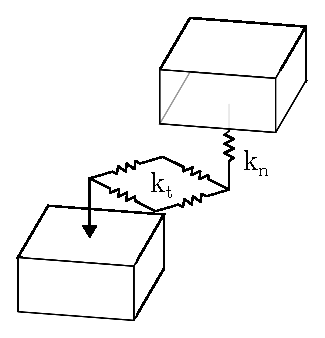
\includegraphics[width=0.5\linewidth]{FIGS/CMODELSCH}}
        \only<3->{\includegraphics[width=\linewidth]{FIGS/TM3DQUADINTSCH}
          \caption{Interface implementation Schematic}}
      \end{figure}
      \begin{itemize}
      \item<1> The normal traction law is given as,
        $$ t_n = \begin{cases} k_n\delta u_n & \delta u_n> 0 \quad (contact)\\0 &
          otherwise \quad (separation) \end{cases} $$
      \vspace{-3cm}\item<2> The incremental tangential traction law in $x$ is given as,
        $$ \Delta t_t^x = \begin{cases} k_t\Delta \delta u_t^x &
          stick\\ 0 & slip\\ -t_{t0}^x & separation \end{cases} $$
      \end{itemize}
    \end{column}
  \end{columns}
\end{frame}

\begin{frame}
  \frametitle{Frequency Response Estimates}
  \only<1>{\framesubtitle{X Direction Excitation (at Sensor 1)}
    \begin{figure}[!h]
      \centering
      \begin{subfigure}{0.5\linewidth}
        \includegraphics[width=\linewidth]{../FIGS/FRFA_WGN_X1}
        \caption{Amplitude}
      \end{subfigure}%
      \begin{subfigure}{0.5\linewidth}
        \includegraphics[width=\linewidth]{../FIGS/FRFP_WGN_X1}
        \caption{Phase}
      \end{subfigure}
      \vspace{-0.25cm}
      \caption{Frequency Response Estimate From White Noise
        Excitation}
      \label{fig:xfresp}
    \end{figure}}
  \only<2>{\framesubtitle{Y Direction Excitation (at Sensor 3)}
    \begin{figure}[!h]
      \centering
      \begin{subfigure}{0.5\linewidth}
        \includegraphics[width=\linewidth]{../FIGS/FRFA_WGN_Y8}
        \caption{Amplitude}
      \end{subfigure}%
      \begin{subfigure}{0.5\linewidth}
        \includegraphics[width=\linewidth]{../FIGS/FRFP_WGN_Y8}
        \caption{Phase}
      \end{subfigure}
      \vspace{-0.25cm}      
      \caption{Frequency Response Estimate From White Noise
        Excitation}
      \label{fig:yfresp}
    \end{figure}}
  \only<3>{\framesubtitle{Z Direction Excitation (at Sensor 2)}
    \begin{figure}[!h]
      \centering
      \begin{subfigure}{0.5\linewidth}
        \includegraphics[width=\linewidth]{../FIGS/FRFA_WGN_Z6}
        \caption{Amplitude}
      \end{subfigure}%
      \begin{subfigure}{0.5\linewidth}
        \includegraphics[width=\linewidth]{../FIGS/FRFP_WGN_Z6}
        \caption{Phase}
      \end{subfigure}
      \vspace{-0.25cm}
      \caption{Frequency Response Estimate From White Noise
        Excitation}
      \label{fig:zfresp}
    \end{figure}}
\end{frame}

\end{document}
%%% Local Variables:
%%% mode: latex
%%% TeX-master: t
%%% End:
